\chapter{Lattice Quantum Chromodynamics}
\label{chap:latticeqcd}

{\red{

    path integral

    discretisation of path integral, summary of steps in a lattice calculation (like, a couple of sentences)

}}

At low energies ($\sim$200MeV and below), QCD becomes non-perturbative, in other words, the coupling $\alpha_s$ becomes $\mathcal{O}(1)$, and an expansion in $\alpha_s$ (as in perturbation theory) will not be dominated by the leading orders \cite{Schwartz:2013pla}. We require an alternative.
\\ \\
The expectation value of an observable $\mathcal{O}$ in a Yang-Mills theory can be expressed as a Euclidean path integral \cite{Lepage:1998dt};
\begin{align}
 \langle \mathcal{O} \rangle = \int \mathcal{D}A\mathcal{D}\psi\mathcal{D}\bar{\psi} \mathcal{O} e^{-S[A,\psi,\bar{\psi}]},
\end{align}
where $A$ is a gauge field, $\psi$($\bar{\psi}$) is an (anti)fermion field, $S$ is the Euclideanised classical action, and $\mathcal{D}$ denotes integration over all configurations of a field. "Euclideanised" refers to a Wick rotation $t\to it$ in $S$. In the perturbative approach, we would expand $\exp(-\text{interacting part of }S )$ resulting in a power series in
the gauge coupling populated by Feynman diagrams.
\\ \\
The other option is to instead carry out the integral directly. This can only be done numerically.
 Since it's not numerically feasible to carry out an infinite number of integrals, one must approximate spacetime as a discrete 4 dimensional lattice with spacing "$a$" between lattice sites, finite spacial volume $L_x^3$ and finite temporal extent $L_t$. The functional integral becomes
\begin{align}
 \int \mathcal{D}A\mathcal{D}\psi\mathcal{D}\bar{\psi} = \prod_{n} \int dU(x_n) d\psi(x_n) d\bar{\psi}(x_n),
\end{align}
where $n$ is a 4-vector with integer components labelling the sites, and $x_n^{\mu} = an^{\mu}$.
This has a second benefit which is to naturally regularize the theory with a momentum cutoff $\Lambda \sim 1/a$ \cite{Lepage:1998dt}. The gauge field has been replaced with the gauge
``link'':
\begin{align}
U_{\mu}(x) \equiv \exp\left(igaA_{\mu}\left(x+{a\hat{\mu}\over2}\right)\right) \in SU(N_c),
\end{align}
$g$ is the gauge coupling, $\hat{\mu}$ is a unit vector in the $\mu$ direction. Parameterizing the gauge fields this way is motivated by the geometrical interpretation of Yang-Mills theories on discrete spacetime and the requirement of exact gauge symmetry \cite{Munster:2000ez}.

\section{Lattice Gauge Fields}

{\red{

    differential geometry in gauge theory, fibre bundles etc.
}}

\subsection{The Wilson Gauge Action}

{\red{

    wilson action
    
}}

\subsection{Improvements}

{\red{

    general idea of symanzik improvements

    the gluon action used in milc code
    
}}

\section{Lattice Fermions}

{\red{

    naive fermion discretisation

}}

The interacting Dirac action is most naively discretised with
\begin{align}
 S_F &= \sum_{x,\mu} \bar{\psi}(x) \gamma_{\mu} \nabla_{\mu} \psi(x) + m\sum_x \bar{\psi}(x) \psi(x),
 \label{eq:naivefermions}
\end{align}
where $\nabla_{\mu}$ is the gauge covariant finite difference operator,
\begin{align}	
	\nabla_{\mu} \psi(x) = {1\over 2a} ( U_{\mu} (x) \psi(x+a\hat{\mu}) - U^{\dagger}_{\mu}(x-a\hat{\mu})\psi(x-a\hat{\mu}) ).
\label{eq:lat_derivative}
\end{align}
In appendix \ref{sec:doublingprob} we describe the doubling problem. This is the observation that the propagator for a fermion obeying \eqref{eq:naivefermions}, $M^{-1}(k)$ has the property
\begin{align}
	M^{-1}(k+{\pi\over a}\zeta) = \gamma_{5\mu} M^{-1}(k) \gamma_{5\mu}
\end{align}
For 16 4-vectors $\zeta_{\mu} \in \mathbb{Z}_2$. This leads to 16 poles in the fermion specturm, therefore 16 distinct excitations (called \textit{tastes}). We require a way of removing the 15 unphysical excitations.


\subsection{The Doubling Problem}

{\red{

    doubling symmetry $\to$ 16 excitations
    
}}

The interacting Dirac action is most naively discretised with
\begin{align}
 S_F &= \sum_{x,\mu} \bar{\psi}(x) \gamma_{\mu} \nabla_{\mu} \psi(x) + m\sum_x \bar{\psi}(x) \psi(x),
 \label{eq:naivefermions}
\end{align}
where $\nabla_{\mu}$ is the gauge covariant finite difference operator,
\begin{align}	
	\nabla_{\mu} \psi(x) = {1\over 2a} ( U_{\mu} (x) \psi(x+a\hat{\mu}) - U^{\dagger}_{\mu}(x-a\hat{\mu})\psi(x-a\hat{\mu}) ).
\label{eq:lat_derivative}
\end{align}
An issue arises with fermions on the lattice, known as the doubling problem. $S_F$ is invariant under a so-called "doubling symmetry", which is generated by
\begin{align}
	\label{eq:doublingsymmetry}
	\psi(x) & \to \mathcal{B}_{\mu} \psi(x) \equiv  (-1)^{x_{\mu}/a} \gamma_{5\mu} \psi(x) \\
	\bar{\psi}(x) & \to \bar{\psi(x)}\mathcal{B}^{\dagger}_{\mu} \equiv (-1)^{x_{\mu}/a} \bar{\psi}(x) \gamma^{\dagger}_{5\mu}
\end{align}
where $\gamma_{5\mu} = i\gamma_{\mu}\gamma_5$. The product space of these form a group of 16 elements $\{\mathcal{B}_{\zeta}\}$, labeled  by vectors $\zeta$ with $\zeta_{\mu}\in \mathbb{Z}_2$ (e.g.the element $\mathcal{B}_{0}\mathcal{B}_{1}$ is labeled by $\zeta=(1,1,0,0)$).
\\ \\
The physical signifiance of this symmetry can be seen when we study it's effect on the action. First, notice that
\begin{align}
	\mathcal{B}_{\mu} \psi(x) & = \gamma_{5\mu} \sum_k \tilde{\psi}(k) e^{i(k+{\pi\over a}\hat{\mu})\cdot x} \\
	& = \gamma_{5\mu} \sum_k \tilde{\psi}(k-{\pi\over a}\hat{\mu})e^{ik\cdot x}
\end{align}
where $k$ is a set of discrete 4-momenta. The action in momentum space can be written as
\begin{align}
	S = \sum_k \bar{\tilde{\psi}}(k) M(k) \tilde{\psi}(k)
\end{align}
after the operation of $\mathcal{B}_{\mu}$ it becomes
\begin{align}
	S \to \sum_k \bar{\tilde{\psi}}(x)(k) \gamma_{5\mu} M(k+{\pi\over a}\hat{\mu})\gamma_{5\mu} \tilde{\psi}(k)
\end{align}
Since we know $S$ is invariant under this transformation, it must be true that $\gamma_{5\mu} M(k+{\pi\over a}\hat{\mu})\gamma_{5\mu} = M(k)$, and therefore
\begin{align}
	M^{-1}(k+{\pi\over a}\hat{\mu}) = \gamma_{5\mu} M^{-1}(k) \gamma_{5\mu}
	\label{eq:doubling}
\end{align}
$M^{-1}$ is the propagator for the fermion field, so \ref{eq:doubling} shows that the spectrum of the fermion is periodic, with a period of $\pi/a$. We expect a pole in $M^{-1}(k)$ where $k \sim m$, where $m$ is the pole mass of the fermion, but there will now be a second pole at $m + \pi/a$. This will be around the natural cutoff imposed by the lattice $1/a$, and any higher poles like $m+2\pi/a$ is far above the cutoff so will not contribute.  
\\ \\
Generalizing this argument to all elements of the doubling symmetry, we see that
\begin{align}
	M^{-1}(k+{\pi\over a}\zeta) = \gamma_{5\mu} M^{-1}(k) \gamma_{5\mu}
\end{align}
leading to 16 poles in the fermion specturm, therefore 16 distinct excitations (called \textit{tastes}).
\\ \\
We now show that there are only 4 tastes in the staggered quark formalism. 
One can isolate a single taste by a block-scaling procedure:
\begin{align}
	\psi^{(\zeta)}(x_B) = \sum_{\delta x_{\mu} \in \mathbb{Z}_2} \mathcal{B}_{\zeta} \psi(x_B + \delta x)
\end{align}
For example, for $\zeta = 0$, it would only contain the original non-doubler taste, since all other poles at $|k|\sim\psi/a$ have been integrated out. For $\zeta \neq 0$, the $\mathcal{B}_{\zeta}$ operator pushes the $\zeta$ doubler to where the $\zeta=0$ taste originally was in $k$ space, then the blocking procedure integrates out the rest. Now writing this isolated taste in terms of $\chi$ we arrive at:
\begin{align}
	\psi^{(\zeta)}(x_B) = \sum_{\delta x_{\mu} \in \mathbb{Z}_2} \Omega(\delta x) \mathcal{B}_{\zeta}(0) \chi(x+\delta x)
\end{align} 
Recall we set $\chi(x) = (\chi_1(x),0,0,0)$. The product $\Omega(\delta x) \mathcal{B}_{\zeta}(0)$ is simply a product of gamma matrices, so can only serve to "scramble" the elements of $\chi$. Then, in the staggered formalism, all 16 tastes $\psi^{(\zeta)}$ amount to only 4 distinguishable fermions: $(\chi_1,0,0,0)$, $(0,\chi_1,0,0)$, $(0,0,\chi_1,0)$, $(0,0,0,\chi_1)$ (with factors of (-1) and $i$).


\subsection{Staggered Quarks}

{\red{

    staggered transformation

    proof that there are only 4 doublers now

    spin-taste basis

}}

There are a number of solutions to this problem. The most straightforward is to modify the action to push the mass of the unwanted tastes above the momentum cutoff, preventing it from effecting the dynamics ("\textit{Wilson fermions}")(\cite{DeGrand:2006zz} ch.6.2). However, actions of this type explicity break Chiral symmetry. Among other issues, this causes additive renormalization of the fermion mass, immensely complicating the renormalization procedure.
\\ \\
Annother approach, known as \textit{staggered quarks}(\cite{DeGrand:2006zz} ch.6.3), partially resolves the doubling issue while retaining chiral symmetry. This is the method we use in our study. Other notable approaches besides Wilson and staggered quarks include \textit{domain wall} \cite{Jansen:1994ym} and \textit{overlap} \cite{Narayanan:2011qj} fermions.
\\ \\
The general idea of staggered fermions is the following.
Redefine the fields according to
\begin{align}
 \psi(x) = \prod_{\mu}(\gamma_{\mu})^{x_{\mu}/a} \chi(x) \equiv \Omega(x) \chi(x)
 \label{eq:staggered}
\end{align}
In terms of the new spinor variables $\chi(x)$, the naive action \eqref{eq:naivefermions} becomes
\begin{align}
  S_F &= \bar{\chi}(x)[\alpha_{\mu}(x) \nabla_{\mu} + m ] \chi(x)
\end{align}
where $\alpha_{\mu}(x) = (-1)^{\sum_{\nu < \mu} x^{\mu}/a}$. The action is now diagonal in spin, leading to 4 decoupled grassman variables with identicle actions and identicle coupling to the gauge field. As a result, $\chi$ propagators (on fixed gauge backgrounds) are spin diagonal:
\begin{align}
	M^{-1}_{\chi}(x,y)[U] = s(x,y)[U] \text{ } 1_{\text{spin}}
\end{align}
One need only to include a single component of $\chi$ in a simulation (i.e. fix $\chi = (\chi_1,0,0,0)$). Then they can compute $M^{-1}_{\chi}(x,y)[U]$ to obtain $s(x,y)$. Then, using the inverse of \eqref{eq:staggered}, $s(x,y)$ can be transformed to a propagator of the original spinors:
\begin{align}
	M_{\psi}^{-1}(x,y)[U] = s(x,y)[U] \Omega(x) \Omega^{\dagger}(y)
\end{align}
This is clearly computationally beneficial. But also, by shaving off the other spinor components, one reduces the number propagating degrees of freedom by a factor of 4. This cuts the number of tastes from 16 down to 4 (this is shown in appendix \ref{sec:doublingprob}).
\\ \\
The remaining multipilcity is tacked in 3 steps:
\begin{enumerate}
	\item
	Ensure only one taste is created and destroyed in the propagator.
	\item
	Minimize the interaction between tastes by modifying the action.
	\item
	Remove contributions of extra tastes in the sea by taking det$M \to \sqrt[4]{\text{det}M}$ in \eqref{eq:MCweight}.
\end{enumerate}
Step 3 can be justified by the following - in the $a\to 0$ limit, det$M$ tends to (det$M^{(0)})^4$, where $M^{(0)}$ is the Dirac oprator for a single taste. Then, taking the 4th root (in principle) reduces the determinant to that of a sea containing 1 taste.

\subsection{Highly Improved Staggered Quarks}

{\red{

    define HISQ

    minimises taste exchange

    removes some tree-level artifacts

}}

\begin{figure}
  \begin{center}
    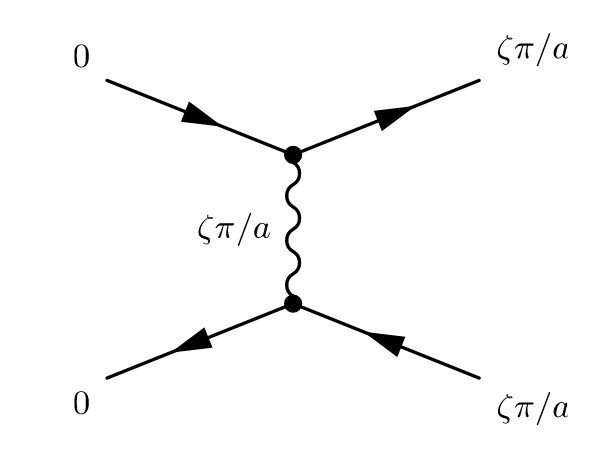
\includegraphics[width=
   0.45\textwidth]{images/tastemixing.jpg}
  \end{center}
  \caption{Taste mixing at tree level.}
  \label{fig:tastemixing}
\end{figure}

Step 2 above is the guiding principle for the action we use in our study, the Highly Improved Staggered Quark action (HISQ). 
\\ \\
Interaction between different tastes ("taste mixing") is dominated by the process in fig. \ref{fig:tastemixing}. In HISQ, this is suppressed by modifying the gauge fields in such a way as to minimize the coupling between a gluon with momentum ${\pi/a}$ and the fermions, in other words, minimize the vertices in fig. \ref{fig:tastemixing}. To this end, one can change the action so that fermions only couple to \textit{smeared} gauge links, in which high frequency exitations have been removed. \\ \\
Define the first and second covariant derivative operators:
\begin{align}
	\nonumber
	\delta_{\rho}U_{\mu}(x) & \equiv {1\over a} \big( U_{\rho} (x) U_{\mu} (x + a\hat{\rho}) U_{\rho}^{\dagger}(x+a\hat{\mu}) \\
	& - U_{\rho}^{\dagger}(x-a\hat{\rho})U_{\mu}(x-a\hat{\rho})U_{\rho}(x-a\hat{\rho}+a\hat{\mu})\big)  \\
	\nonumber
	\delta_{\rho}^{(2)} U_{\mu}(x) & \equiv {1\over a^2} \big( U_{\rho}(x+a\hat{\rho})U^{\dagger}_{\rho}(x+a\hat{\mu}) \\
	\nonumber	
	& - 2U_{\mu}(x) \\
	& + U_{\rho}^{\dagger}(x-a\hat{\rho})U_{\mu}(x-a\hat{\rho})U_{\rho}(x - a\hat{\rho} + a\hat{\mu}) \big)
\end{align}
With this we can define the smearing operator;
\begin{align}
	\mathcal{F}_{\mu} = \prod_{\rho\neq\mu} \left( 1 + {a^2 \delta^{(2)}_{\rho}\over 4} \right)
\end{align}
HISQ uses two different smeared gauge fields defined by;
\begin{align}
	X_{\mu}(x) &\equiv \mathcal{U} \mathcal{F}_{\mu} U_{\mu}(x) \\
	W_{\mu}(x) &\equiv \left(\mathcal{F}_{\mu} - \sum_{\rho\neq\mu}{a^2(\delta_{\rho})^2\over 2} \right) \mathcal{U} \mathcal{F}_{\mu} U_{\mu}(x)
	\label{eq:gaugesmearing}
\end{align}
where $\mathcal{U}$ is a re-unitarization operator. The HISQ action can then be written as:
\begin{align}
	S_{\text{HISQ}} = \sum_{x} \bar{\psi}(x) \left( \gamma\cdot \left( \nabla_{\mu}(W) - {a^2\over 6}(1+\epsilon_{\text{Naik}})\nabla^3_{\mu}(X) \right) + m \right) \psi(x)
\end{align}
Where $\nabla_{\mu}(Z)$ is the covariant derivative \eqref{eq:lat_derivative} with gauge links repaced with $Z$. This action in fact not only removes tree level interactions like fig. \ref{fig:tastemixing}, but also all taste mixing interactions at 1-loop. The $\nabla^3_{\mu}$ term is introduced to remove "lattice artifacts", i.e. it reduces the size of $\mathcal{O}(a)$ terms in the $a\to 0$ limit of the action. In the same spirit, $\epsilon_{\text{Naik}}$ is fixed according to the constraint
\begin{align}
	\lim_{\underline{p}\to 0} {E^2(\underline{p})-m^2\over \underline{p}^2} = 1
\end{align}
where $E(\underline{p})$ obeys the dispersion relation from HISQ. The motivation for the specific smearing of the gauge fields \eqref{eq:gaugesmearing}, and more details on HISQ in general, are given in \cite{Follana:2006rc}.

\section{Dealing with Heavy Quarks}

{\red{
    heavy quarks are hard, because they fall inbetween lattice sites. $b$ is almost within reach.
}}

\subsection{Heavy HISQ}

{\red{

    extrapolation to physical $b$

    general principles of fit function (hqet etc)

}}

\subsection{Lattice NRQCD}

{\red{

    this can be done at the physical $m_b$, rest mass chopped out

    write out lattice NRQCD action

    define lattice NRQCD currents

}}
